%============================ Project Managenent Document ================================
% define document class
\documentclass[
	a4paper               % paper format
%	,10.5pt               % fontsize
	,BCOR=0mm            % Binding correction
	,bibliography=totoc   % If enabled add bibliography to TOC
	,listof=totoc         % If enabled add lists to TOC
%	,bilingual
	,monolingual
	,twoside=false
]{bfhthesis}              % KOMA-script report

\setcounter{secnumdepth}{4}

\PassOptionsToPackage{hyphens}{url}\usepackage[
	hidelinks,
	pdfusetitle,
]{hyperref}
\usepackage{tikzducks}
\usepackage{amsmath}
\usepackage{listings}

\LoadBFHModule{boxes}

\colorlet{punct}{red!60!black}
\definecolor{background}{HTML}{EEEEEE}
\definecolor{delim}{RGB}{20,105,176}
\colorlet{numb}{magenta!60!black}

\lstdefinelanguage{json}{
    basicstyle=\normalfont\ttfamily,
    numbers=left,
    numberstyle=\scriptsize,
    stepnumber=1,
    numbersep=8pt,
    showstringspaces=false,
    breaklines=true,
    frame=lines,
	postbreak=\mbox{\textcolor{red}{$\hookrightarrow$}\space},
    backgroundcolor=\color{background},
    literate=
      {:}{{{\color{punct}{:}}}}{1}
      {,}{{{\color{punct}{,}}}}{1}
      {\{}{{{\color{delim}{\{}}}}{1}
      {\}}{{{\color{delim}{\}}}}}{1}
      {[}{{{\color{delim}{[}}}}{1}
      {]}{{{\color{delim}{]}}}}{1},
}

\lstdefinelanguage{canon}{
    basicstyle=\normalfont\ttfamily,
    numbers=left,
    numberstyle=\scriptsize,
    stepnumber=1,
    numbersep=8pt,
    showstringspaces=false,
    breaklines=true,
    frame=lines,
    backgroundcolor=\color{background},
	postbreak=\mbox{\textcolor{red}{$\hookrightarrow$}\space},
}

\hyphenation{ve-ri-fi-ca-ti-on}

\begin{document}

\frontmatter

\title{Bachelor's Thesis}
\subtitle{Unlinkability of Verifiable Credentials in a practical approach: Project Management}
\author{Joël Gabriel Robles Gasser}
\institution{Bern University of Applied Sciences}
\department{Engineering and Computer Science}
\institute{Computer Science}
\version{1.0}
\date{June 13, 2024}
\advisor{Prof. Dr. Annett Laube\and Prof. Dr. Reto Koenig}
\expert{Dr. Andreas Spichiger}
\degreeprogram{Bachelor of Science in Computer Science}

%----------------  BFH tile page   -----------------------------------------
\maketitle


%------------ TABLEOFCONTENTS ----------------
\tableofcontents

%------------ START MAIN PART ----------------
\mainmatter

\chapter{Risks}
In this chapter, we define risks that may happen in this thesis.

\section{Project Risks}

\subsection{VC}
\begin{itemize}
	\item Risk: There is the possibility that the structure of VCs might break the unlinkability of BBS
	\item Solution: If that is the case, the structure of VCs needs to be reworked so there is no linkability
	\item Possibility: Low
\end{itemize}

\subsection{OIDC4VP}
\begin{itemize}
	\item Risk: There is the possibility that the implementation of OIDC4VP leaks data
	\item Solution: If that is the case, the structure of the OIDC4VC protocol needs to be reworked so there are no more data leaks
	\item Possibility: Low
\end{itemize}

\subsection{OIDC4VP}
\begin{itemize}
	\item Risk: There is the possibility that the implementation of OIDC4VP leaks data
	\item Solution: If that is the case, the structure of the OIDC4VC protocol needs to be reworked so there are no more data leaks
	\item Possibility: Low
\end{itemize}
\begin{itemize}
	\item Risk: There is the possibility that the implementation of OIDC4VP breaks the unlinkability of BBS
	\item Solution: If that is the case, the structure of the OIDC4VP protocol needs to be reworked so there is no linkability
	\item Possibility: Medium
\end{itemize}

\subsection{Pseudonyms}
\begin{itemize}
	\item Risk: There is the possibility that the implementation of pseudonyms breaks the unlinkability of BBS
	\item Solution: If that is the case, the structure of pseudonyms needs to be reworked, so there is no linkability
	\item Possibility: Low
\end{itemize}

\subsection{Link Secrets}
\begin{itemize}
	\item Risk: There is the possibility that the implementation of Link Secrets breaks the unlinkability of BBS
	\item Solution: If that is the case, the implementation of the Link Secrets needs to be reworked, so there is no linkability
	\item Possibility: Medium
\end{itemize}
\begin{itemize}
	\item Risk: There is the possibility that the implementation of Link Secrets allows the holder of multiple VCs to link them together on a different Secret
	\item Solution: If that is the case, the implementation of the Link Secrets needs to be reworked, so that this is no longer possible
	\item Possibility: Low
\end{itemize}

\section{Environmental risks}

\subsection{Sickness}
\begin{itemize}
	\item Risk: There is a possibility that I might become sick
	\item Solution: If the sickness is less than 1 week, there is a buffer in the project plan at the end of the semester for that. If it's more than 1 week, there is a chance that the project would need to be moved to another semester
	\item Possibility: Medium
\end{itemize}

\subsection{Hardware}
\begin{itemize}
	\item Risk: There is a possibility that the hardware used (laptop) may break due to unknown reasons
	\item Solution: The deliverables are backed up to GitHub and mirrored to the BFH-TI GitLab. There is also a backup on other hardware. There also backup hardware if the main hardware would break
	\item Possibility: Low
\end{itemize}
\begin{itemize}
	\item Risk: There is the possibility that the backups are not accessible
	\item Solution: In that case, there is also a backup on different devices
	\item Possibility: Low
\end{itemize}

\subsection{Project Plan/Ideas}
\begin{itemize}
	\item Risk: There is the possibility that the project plan is bad, so that the planned time frames are too short
	\item Solution: In that case, there is 1 week buffer at the end of the semester. If that is not enough time, then there needs to be an explanation in the documentation why that happened
	\item Possibility: Medium
\end{itemize}
\begin{itemize}
	\item Risk: There is the possibility that the expert of the project may bring new ideas into the project
	\item Solution: If those ideas further the project goals, they may be added to the project plan. In that case the project plan needs to be reworked
	\item Possibility: Low
\end{itemize}


\chapter{Meetings}
In this semester I've attended many meetings with different parties: with my advisors, with the expert and with the BBS working group.\\

\noindent
\textbf{Meetings with advisors:}\\
Nearly each week I met with my advisors. In those meetings, we discussed my new findings, about the sprint results or about the documentation. Those meetings helped me a lot to stay more or less within my sprint deadlines, and I learned a lot of things about researching and documenting.\\

\noindent
\textbf{Meetings with expert:}\\
This semesters, I had three meetings with the expert. The first meeting was all about the project management, the goal and the first results. The second meeting was around the half way mark of the semester, where I presented a first version of the my defense, with results up to that point. I got some feedback, which I used to improve the defense. Then there was a third meeting one week before the due date, where I presented the full defense as a test run. On that date there were also three other listeners that were interested in the technologies. After the presentation, I got feedback from all of them, which I can use to again improve the defense.\\

\noindent
\textbf{Meetings with the BBS working group:}\\
Nearly each monday evening, the BBS working group meets online to talk about new issues, new ideas or updates to the BBS specifications. I participated in many of those meetings and asked questions based on my current findings, to better understand the whole picture.


\chapter{Project Management}
In this chapter the project management which was done in this semester is thematized.
In figure \ref{fig:roadmap} one can see the roadmap created for this thesis. This roadmap contains all the planned sprints for the whole project.\\

I've used Scrum for the project management. All the tasks (besides the documenting and meetings) were split up into one- or two-week sprints. At the end of each sprint, I looked back on what was done within that timeframe and used the new knowledge for the sprint. Using Scrum as my project management framework helped me to change directions when something unexpected happened, and thus assisted me in staying organized.

\newpage
\begin{figure}[h]
	\centering
	\rotatebox[origin=c]{270}{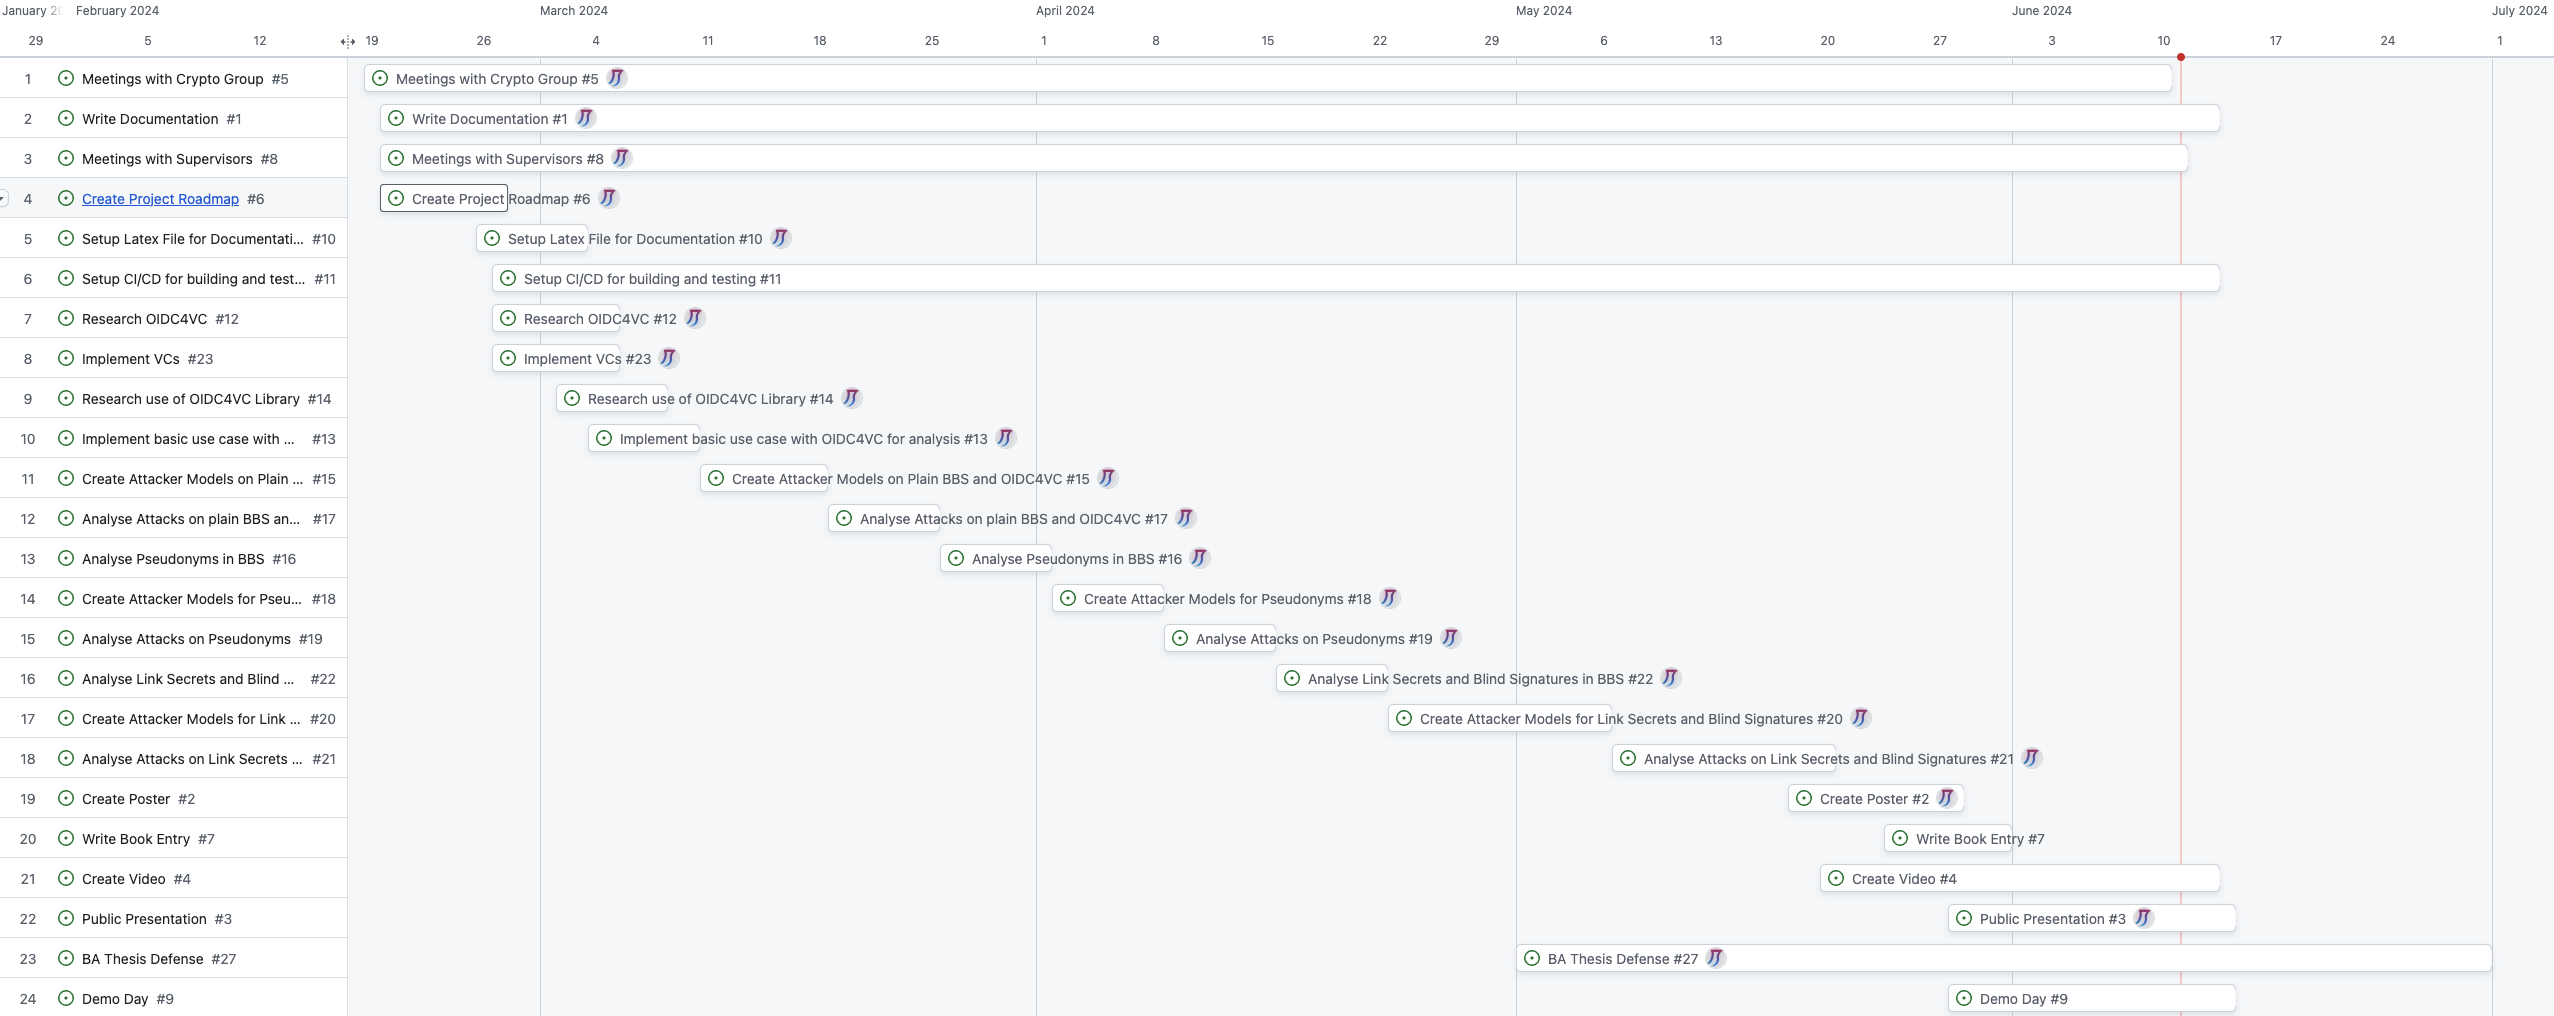
\includegraphics[width=22cm]{./img/projectgraph.png}}
	\label{fig:roadmap}
	\caption{Roadmap}
\end{figure}


\chapter{Found Issues}
While researching for this thesis, many issues were found. This chapter summarizes all the raised issues/written mails.

\section{Github Issues}
These are the issues that were reported in the \textit{Data Integrity BBS Cryptosuites v1.0}\cite{bbsvc} GitHub Repository.\\

\noindent
\textbf{Typo \& missing check}\\
see: \url{https://github.com/w3c/vc-di-bbs/issues/154}\\
In this issue I mentioned a typo. I also mentioned that there is a missing check for a value in an object, as if that value is empty it could raise an error.
The typo was fixed, but the check was not added.\\

\noindent
\textbf{Missing attributes}\\
see: \url{https://github.com/w3c/vc-di-bbs/issues/155}\\
In this issue I mentioned that some attributes used in the algorithm were not passed as parameters. At the same time the authors were changing where all the parameters come from, as the part of the addition of optional features. Error was fixed with the optional features update.\\

\noindent
\textbf{Missing reference}\\
see: \url{https://github.com/w3c/vc-di-bbs/issues/157}\\
In this issue I noted that there was a missing reference to a used algorithm. After searching for a bit, I found that algorithm defined in an other specification. The error was fixed a standalone pull request.\\

\noindent
\textbf{Missing reference: The second}\\
see: \url{https://github.com/w3c/vc-di-bbs/issues/163}\\
Same as in the above mentioned issue, there was a missing reference. At the same time, the wrong algorithm was called. The called algorithm has been corrected and the reference was added, but the pull request was not approved yet.\\
\newpage

\noindent
\textbf{Unused variables}\\
see: \url{https://github.com/w3c/vc-di-bbs/issues/164}\\
In an algorithm, a variable was defined, but never used. The error was corrected, but the pull request was not accepted yet.\\

\noindent
\textbf{Typo \& missing information}\\
see: \url{https://github.com/w3c/vc-di-bbs/issues/166}\\
There was another small typo, which was changed with the next pull request. There was also the problem of how to retrieve the public key, as it is used as an input to an algorithm. This information was also added in the same pull request but was not accepted and merged yet.\\

\noindent
\textbf{Add SHA-3}\\
see: \url{https://github.com/w3c/vc-di-bbs/issues/162}\\
In the Data Integrity BBS Cryptosuites\cite{bbsvc} specification, SHA-256 is used for all hashing operations. I suggested adding the information that SHA-3 would also be a possibility, as the BBS specification also allows hashing with a kmac. This suggestion was rejected, the reason being that a big part of the internet is using SHA-256 and thus the implementation using SHA-256 instead of SHA-3 would be easier.


\section{Written Mails}
While researching OIDC4VP, in the chapters 11.5 and 6 of OpenID for Verifiable Presentations \cite{oidc4vp} it wasn't stated in where the nonce value and the client\_id values should be included. After contacting the authors of the specification, Olivier Terbu responded with the instruction where to add these values in the VP.


\chapter{Problems}
In this chapter the problems that came up while researching and writing this thesis are mentioned.\\

\noindent
\textbf{Sickness}\\
During the project, I was sick twice. Both times for around a week. Although there was a buffer for being sick for one week, the second time shortened my timeframe in which I could work on the thesis.\\

\noindent
\textbf{Extensive Specification}\\
\textit{Verifiable Credentials Data Model v2.0}\cite{verifiable-credentials} is a very extensive specification. There are many optional features that are not really needed for this thesis. So it took some time to determine which features should be used.\\

\noindent
\textbf{Unclear Specification}\\
The \textit{Data Integrity BBS Cryptosuites v1.0}\cite{bbsvc} specification was very unclear. I did not really understand what the different algorithms did, or what the required inputs where. I used Greg Bernsteins, one of the authors, implementation to understand each step in the algorithms. I needed to write up the specification in a way that was more or less understandable. This used a lot of time and was not planned, thus leaving less time for other parts of the thesis.\\

\noindent
\textbf{Documentation}\\
For me, the documentation was the biggest problem of the whole thesis. It is very hard for me to write up something that reads more or less ok. Therefore, many revisions were needed, which used up way more time than expected. So at the end I needed more than double the time than I planned for the documentation alone.


\bibliographystyle{plain}
\bibliography{refs}



\end{document}
